\section{Мета роботи}
Отримати та закріпити знання про внутрішнє подання
інтегрованих структур даних у мовах програмування.

\noindent
\textbf{Теми для попередньої роботи:}
\begin{itemize}
    \item фізичне та логічне подання даних;
    \item інтегровані типи даних;
    \item вирівнювання даних.
\end{itemize}


\section{Завдання}
Написати програму, яка виводить на екран внутрішнє подання структури з варіантною частиною та з бітовими полями,
а також масиву структур. Перелік властивостей та відповідні типи полів для об’єктів з
табл. 4.1 обрати за своїм розсудом.

Дослідити, як виконується вирівнювання даних та полів структури.

Порівняти час доступу до даних з вирівнюванням та за умови відсутності вирівнювання.
За результатами роботи підготувати звіт з лабораторної роботи, де навести отримані результати та дати щодо них пояснення, зробити висновки.

\begin{figure}[h!]
    \centering
    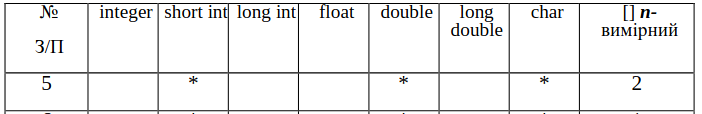
\includegraphics[width=.9\textwidth]{\reportDirectory/var.png}
    \caption{Завдання за варіантом (\variant)}
    \label{fig:task}
\end{figure}


\section{Хід виконання}
Для виконання завдання було обрано мову Rust.
Увесь код також додатково був розміщений в GitHub репозитарії: \href{https://github.com/blackgolyb/algos-labs}{https://github.com/blackgolyb/algos-labs}.


\newpage
\subsection{Визначення структур даних}
Для завдання визначимо структури для дослідження.
Також скористаємося макросом для \verb|impl_show_bytes| того,
щоб відображати структуру в байтовому вигляді.

А також розглянемо як в Rust можна контролювати вирівнювання даних.
Для цього в Rust використовується \textit{repr}.
Для того, щоб досягти врівнювання як в C треба використати \verb|#[repr(C)]|,
а для того, щоб повністю позбутися вирівнювання треба використати \verb|#[repr(C, packed(1))]|.

\noindent
Код програми:
\begin{lstlisting}[language=Rust, style=colouredRust]
use std::mem::ManuallyDrop;

use crate::libs::bytes::{impl_show_bytes, show, ShowBytes};

pub struct StandardPc {
    pub filed1: u8,
    pub filed2: i32,
    pub filed3: u8,
}

pub struct StandardTable {
    pub filed1: u8,
    pub filed2: i32,
}

pub union StandardUnion {
    pub pc: ManuallyDrop<StandardPc>,
    pub table: ManuallyDrop<StandardTable>,
}

pub struct Standard {
    pub kind: StandardUnion,
    pub for_child: bool,
    pub cooperative: bool,
}
impl_show_bytes!(Standard);
\end{lstlisting}


Тепер реалізуємо код який буде робити порівняння всіх типів структур: з вирівнюванням, без вирівнювання, а також додатково розглянемо стандартну структуру Rust.

\noindent
Код програми:
\begin{lstlisting}[language=Rust, style=colouredRust]
use std::mem::ManuallyDrop;
use std::time::Instant;

use super::variants::aligned::{Aligned, AlignedPc, AlignedTable, AlignedUnion};
use super::variants::packed::{Packed, PackedPc, PackedTable, PackedUnion};
use super::variants::sandard::{Standard, StandardPc, StandardTable, StandardUnion};
use crate::libs::bytes::ShowBytes;

macro_rules! create_pc {
    ($st:ident, $u:ident, $pc:ident) => {
        $st {
            for_child: false,
            cooperative: true,
            kind: $u {
                pc: ManuallyDrop::new($pc {
                    filed1: 12,
                    filed2: !0,
                    filed3: 26,
                }),
            },
        }
    };
}

macro_rules! create_table {
    ($st:ident, $u:ident, $table:ident) => {
        $st {
            for_child: false,
            cooperative: true,
            kind: $u {
                table: ManuallyDrop::new($table {
                    filed1: 12,
                    filed2: !0,
                }),
            },
        }
    };
}

macro_rules! display {
    ($t:ident, $pc:ident, $table:ident) => {
        println!("{:=^30}", stringify!($t));
        println!("size of {}", size_of::<$t>());
        print!("PC bytes representation: ");
        $pc.show_bytes();
        println!();
        print!("    for_child: ");
        $pc.for_child.show_bytes();
        println!();
        print!("    cooperative: ");
        $pc.cooperative.show_bytes();
        println!();
        unsafe {
            let f1 = $pc.kind.pc.filed1;
            let f2 = $pc.kind.pc.filed2;
            let f3 = $pc.kind.pc.filed3;
            print!("    filed1: ");
            f1.show_bytes();
            println!();
            print!("    pc filed2: ");
            f2.show_bytes();
            println!();
            print!("    pc filed3: ");
            f3.show_bytes();
            println!();
        }

        println!();

        print!("Table bytes representation: ");
        $table.show_bytes();
        println!();
        print!("    for_child: ");
        $pc.for_child.show_bytes();
        println!();
        print!("    cooperative: ");
        $pc.cooperative.show_bytes();
        println!();
        unsafe {
            let f1 = $pc.kind.table.filed1;
            let f2 = $pc.kind.table.filed2;
            print!("    filed1: ");
            f1.show_bytes();
            println!();
            print!("    table filed2: ");
            f2.show_bytes();
            println!();
        }

        let n = 10000000;

        let now = Instant::now();
        for _ in 0..n {
            unsafe {
                $pc.kind.pc.filed3;
            }
            $pc.for_child;
            $pc.cooperative;
        }
        println!("PC time: {} ns  repeats: {n}", now.elapsed().as_nanos().to_string());

        let now = Instant::now();
        for _ in 0..n {
            unsafe {
                $table.kind.table.filed2;
            }
            $table.for_child;
            $table.cooperative;
        }
        println!("Table time: {} ns  repeats: {n}", now.elapsed().as_nanos().to_string());
        println!("{:=^30}\n", "");
    };
}

pub fn main() {
    let packed_pc = create_pc!(Packed, PackedUnion, PackedPc);
    let packed_table = create_table!(Packed, PackedUnion, PackedTable);

    let aligned_pc = create_pc!(Aligned, AlignedUnion, AlignedPc);
    let aligned_table = create_table!(Aligned, AlignedUnion, AlignedTable);

    let sandard_pc = create_pc!(Standard, StandardUnion, StandardPc);
    let sandard_table = create_table!(Standard, StandardUnion, StandardTable);

    display!(Packed, packed_pc, packed_table);
    display!(Aligned, aligned_pc, aligned_table);
    display!(Standard, sandard_pc, sandard_table);
}
\end{lstlisting}


\newpage
\subsection{Приклад роботи програми}
Для кращого розуміння зображено на картинках відповідність між байтами кольором.
Білим кольором позначено невикористовувану пам'ять.
\begin{figure}[h!]
    \centering
    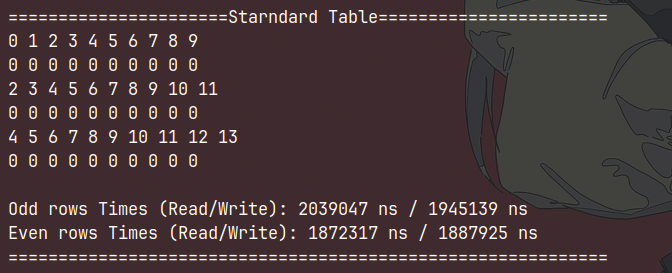
\includegraphics[width=\textwidth]{\reportDirectory/img1.png}
    \caption{Приклад роботи для структури без вирівнювання}
    \label{fig:task}
\end{figure}
\begin{figure}[h!]
    \centering
    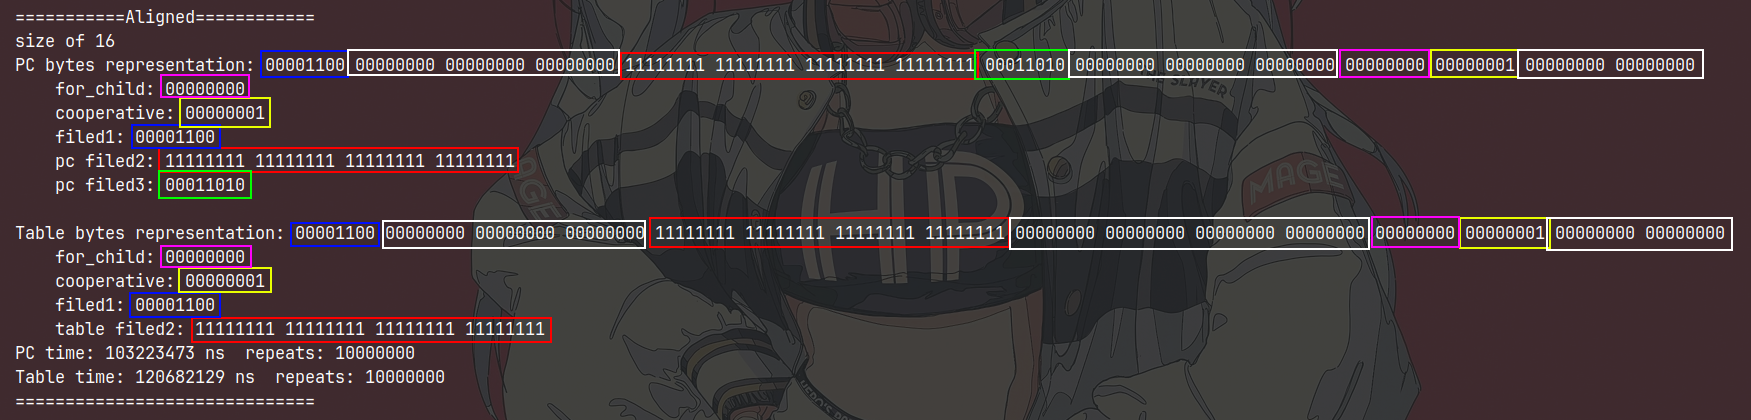
\includegraphics[width=\textwidth]{\reportDirectory/img2.png}
    \caption{Приклад роботи для структури з вирівнювання як в С}
    \label{fig:task}
\end{figure}
\begin{figure}[h!]
    \centering
    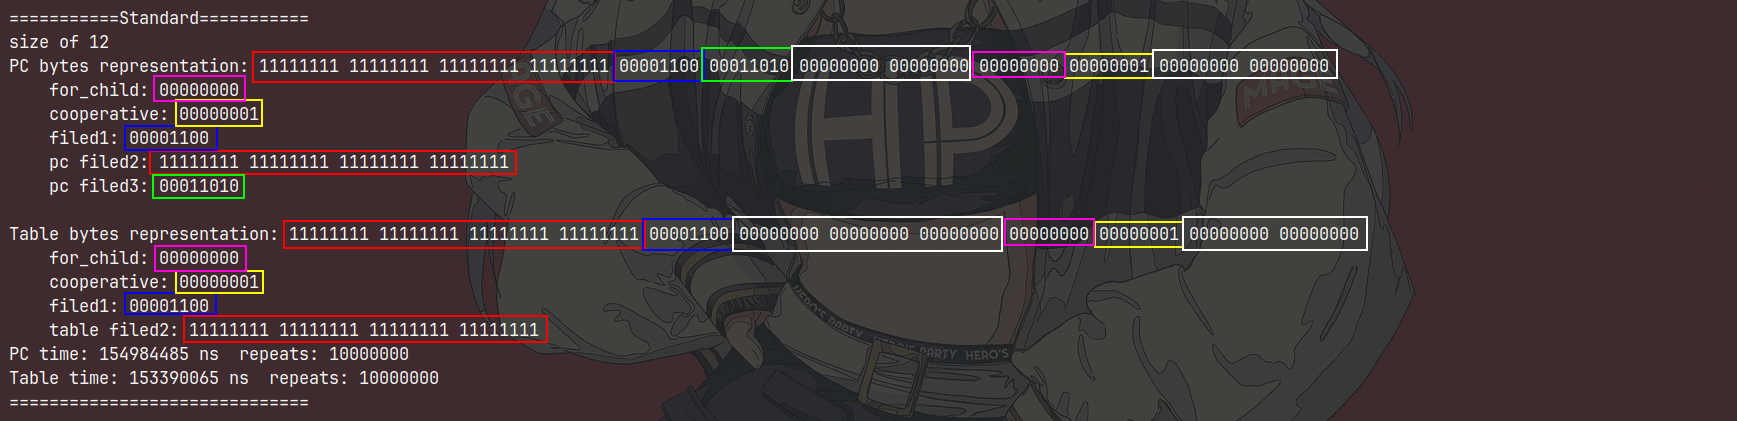
\includegraphics[width=\textwidth]{\reportDirectory/img3.png}
    \caption{Приклад роботи для структури з вирівнювання як в Rust}
    \label{fig:task}
\end{figure}


\newpage
\section{Висновки}
В ході виконання лабораторної робити було порівняно бітове подання структур,
а також час доступу до їх полів. Після багаторазового порівняння часу звертання до полів вирівняних та не вирівняних структур,
не було помічено якоїсь різниці з поправкою на похибку.
